\documentclass[12pt,a4paper]{report}
\usepackage[utf8]{inputenc}
\usepackage[spanish]{babel}
\usepackage{amsmath}
\usepackage{amsfonts}
\usepackage{amssymb}
\usepackage{makeidx}
\usepackage{graphicx}
\usepackage{lmodern}
\usepackage{kpfonts}
\usepackage[left=2cm,right=2cm,top=2cm,bottom=2cm]{geometry}
\author{Diego Armando Becerra Iñiguez}
\title{Algoritmo de Denavit-Hartenberg}
\begin{document}
\maketitle 
\section{Introducción}
Existe un estudio en la robótica, existe un algoritmo, llamado \textbf{El algoritmo de Denavit-Hartenberg}, que nos ayuda a establecer los sistemas de referencia para cada uno de los eslabones con los que cuenta el robot.
\section{Algoritmo}
\subsection{Paso 0}
Determinar el número de eslabones y el número de articulaciones. Utilizaremos un hipotetico caso el cual tiene que el número de eslabones es n+1, con n=7 y el número de articulaciones es n; por lo tanto hay 8 eslabones en este ejemplo. Para los eslabones, la numeración comienza en 0, el eslabón 0 es la base y el eslabón n=7 es el efector final. Las articulaciones comienzan a numerarse en 1.
\begin{figure}[hbtp]
\centering
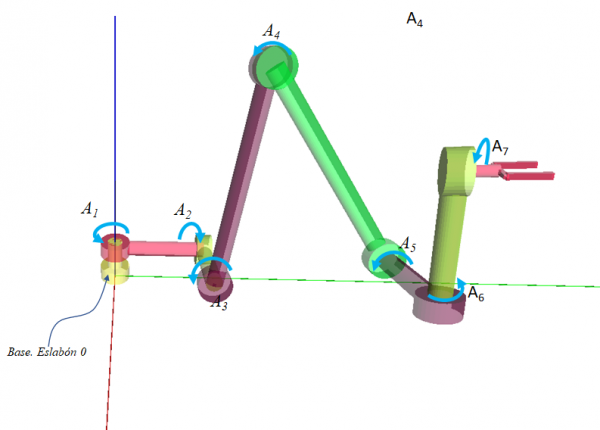
\includegraphics[width=10cm]{1.png}
\caption{Identificación de las articulaciones del robot,siempre hay un eslabón más que el numero de articulaciones.}
\end{figure}
\subsubsection{Caso especial. Base (eslabón 0)}
\textbf{Determinar la dirección del eje $z_{0}$}.
El eje $z_{0}$ se escoge de tal forma que este alineado (es decir además de paralelo debe estar en la misma línea) con el eje de la articulación $A_{1}$ (figura 3), el origen del sistema referencia $B_{0}$(base) se sitúa en cualquier punto del eje $z_{0}$.
Los ejes \textbf{$x_{0}$},\textbf{$y_{0}$},\textbf{$z_{0}$}del sistema de referencia \textbf{$B_{0}$} situado en el eslabón 0(base) son fijos(no rotan), se encogen de tal manera que sea un sistema que \textbf{obedece a la regla de la mano derecha}(figura 2).

\begin{figure}[hbtp]
\centering
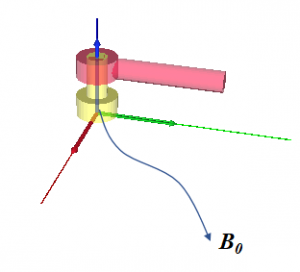
\includegraphics[width=10cm]{2.png}
\caption{Eje z de eslabón 0 (base) que coincide con la dirección de la siguiente articulación}
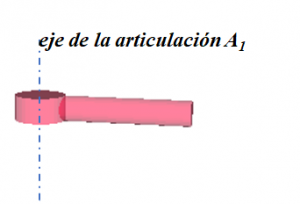
\includegraphics[width=10cm]{3.png}
\caption{Articulación A1}
\end{figure}

\subsubsection{Caso especial. Efector final}
\paragraph{(eslabón n)}
Para el último eslabón la elección del sistema de referencia $B_{n}$ el eje $x_{n}$ debe ser perpendicular al eje $z_{n-1}$;si la articulación es revoluta al eje $z_{n}$ está alineado (coincide) con el eje $z_{n-1}$ (ver figura 8).
\subsection{Paso 1}
Para cada eslabón  i=1,2,3…n-1 ( en este ejemplo n-1=6, el i=0 es la base y para el efector final i=7, véase paso 0)  hay tres pasos a realizar para elegir la dirección $z_{i}$ y la dirección $x_{i}$, con ello el eje $y_{i}$ se elige simplemente de tal forma que el sistema de referencia $B_{i}$ sea un sistema que obedece a la regla de la mano derecha(dextrógiro).

\textbf{Determinar la dirección de los ejes $z_{i}$ con i=1,2,3...n-1.}

 El eje $z_{i}$ se escoge de tal forma que este alineado(en la misma linea) con el de la articulación $A_{i+1}$.
 
 Cada eje $z_{i}$ esta montado sobre el eslabon i.
 
 Para el eslabón 1, según el robot SSRMS de ejemplo en estudio, a continuación se muestra la configuración del eslabón 1 con el eslabón 2, aún sin representar el eje $z_{i}$. 
\begin{figure}[hbtp]
\centering
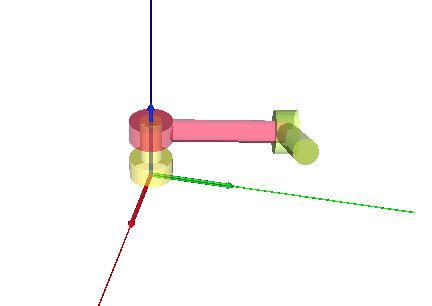
\includegraphics[width=7cm]{4.png}
\caption{Aún no se ha especificado la dirección del eje z1 montando en el eslabón 1}
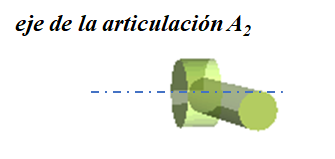
\includegraphics[width=7cm]{5.png}
\caption{Eslabón 2}
\end{figure}
De acuerdo con la figura 5, el eje z del eslabón 1 queda como se muestra en la figura 6, es decir, de tal manera que al ensamblar el robot el eje $z_{1}$ esté alineado con el eje de la articulación $A_{2}$.
\begin{figure}
\centering
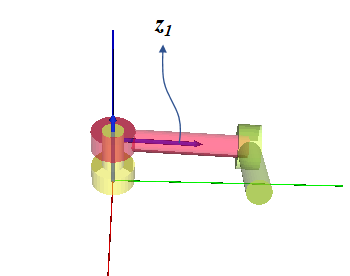
\includegraphics[width=6cm]{6.png}
\caption{Ilustración de la elección correcta del eje z del eslabón 1.}
\end{figure}
\\\\

Continuando de esta manera el conjunto de ejes $z_{i}$con i=0,1,2,3…n-1, se ilustra en la figura 7.
\begin{figure}[hbtp]
\centering
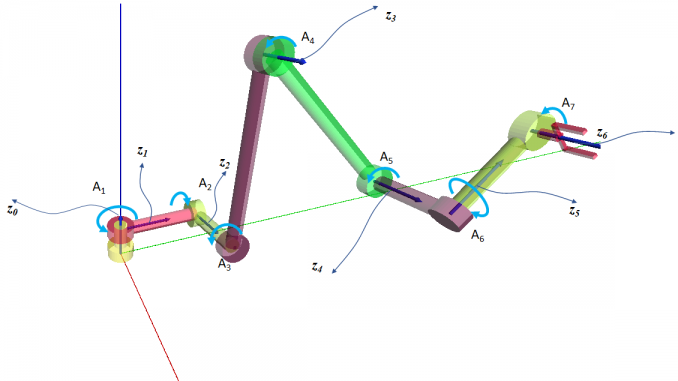
\includegraphics[width=7cm]{7.png}
\caption{Ejes zi alineado con eje de articulación Ai+1}
\end{figure}
\subsection{Paso 2}
\textbf{Determinar la dirección de los ejes $x_{i}$ con i=1,2,3...n-1}
\subsubsection{Caso 1}
Si los ejes $z_{i} y z_{i-1}$ se intersecan, la dirección del eje $x_{i}$ esta dada por la dirección del vector $x_{i}=z_{i}x \;z_{i-1}$.

\textbf{Para el caso 1, donde ocurre tal intersección se coloca el origen del sistema de referencia $B_{i}$}.
De la figura 8, observe que este caso se cumple para los ejes $x_{i}$ con i=1,2,5,n-1.
\begin{figure}[hbtp]
\centering
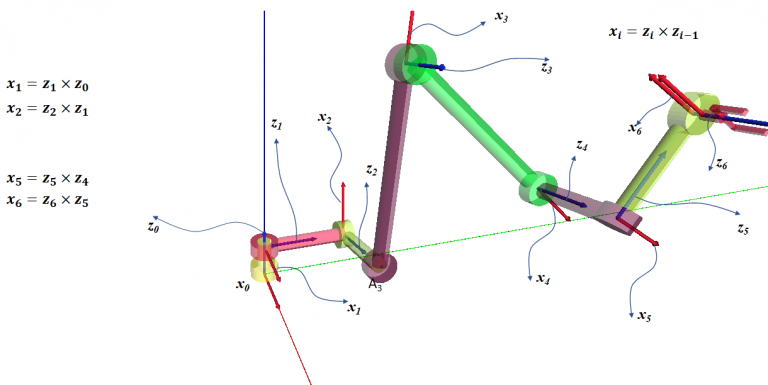
\includegraphics[width=10cm]{8.png}
\caption{}
\end{figure}
\subsubsection{Caso 2}
Si los ejes $z_{i} y z_{i-1}$ son paralelos, hay un número infinito de normales comunes,  escoja alguna de ellas (la más adecuada o cómoda), la dirección del eje $x_{i}$ esta dada por la dirección de lo normal común que eligió, ésta se dirige del eje $z_{i-1}$ al eje $z_{i}$.

De la figura 8, observe que los ejes $z_{2} y z_{3}$, así como los ejes $z_{3} y z_{4}$ son paralelos y por lo tanto esto implica que este caso aplica para definir  la dirección de los ejes $x_{3}\; y \;x_{4}$ 

\subsubsection{Caso 3}
Si los ejes $z_{i}\; y z_{i-1}$ no son paralelos ni se intersecan, la dirección del eje $x_{i}$ esta dada por la dirección de la normal común entre dichos ejes, esta  se dirige del eje $z_{i-1}$ al eje $z_{i}$ en el robot SSRMS no ocurre en este caso.

Para el caso 2 y 3 el origen del sistema de referencia $B_{i}$ se elige donde ocurre la intersección de la normal común de los ejes $z_{i}$ y $z_{i-1}$ con el eje  de la articulación $A_{i+1}$.

En la figura 9 se ilustra la ubicación de los orígenes para cada uno de los sistemas de referencias ${B_{i}}$ con i=1,2,…,n-1; observe que el origen $B_{3}$ se ubica en la intersección del eje de la articulación $A_{4}$ con la normal común entre el eje $z_{2} \;y\; z_{3}$. Análogamente, el origen $B_{4}$ se ubica en la intersección del eje de la articulación $A_{5}$ con la normal común entre el eje $z_{3}\;y \;z_{4}$.

\begin{figure}[hbtp]
\centering
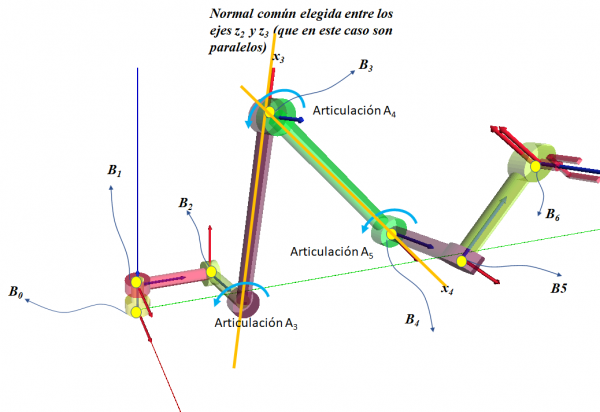
\includegraphics[width=9cm]{9.png}
\caption{La elección de los orígenes se ha realizado según el caso correspondiente. Observe que no siempre se coloca un origen en cada articulación.}
\end{figure}

Con la elección de los origenes ${B_{i}}$ así como de los ejes $z_{i}\; y \; x_{i}$(el eje $y_{i}$) se encuentra fácilmente, ver paso 3)ya se puede comenzar a diseñar y a orientar cada pieza en el sistema de referencia del modelado (sistema de referencia local).

Durante el diseño de la pieza, debe conocerce a priori la dirección del eje de la articulación siguiente, de esta manera el eje z en el sistema de referencia local (donde se modela la pieza), una vez que se ensambla el robot,  debe estar alineado con el eje de la articulación siguiente (para la base ver figura 10 y para eslabón 1 ver figura 12).
\begin{figure}[hbtp]
\centering
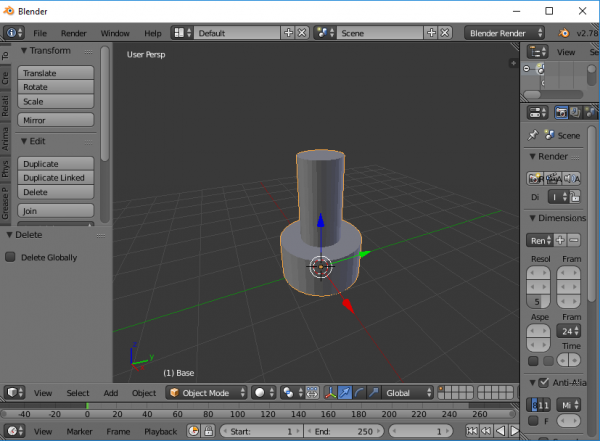
\includegraphics[width=7cm]{10.png}
\caption{Diseño correcto de la base, observe el sistema de referencia local (rojo eje X, verde eje Y, azul eje Z). Al esamblar el robot el eje z de este eslabón 0  coincide con el eje de la articulación A1}
\end{figure}
\begin{figure}[hbtp]
\centering
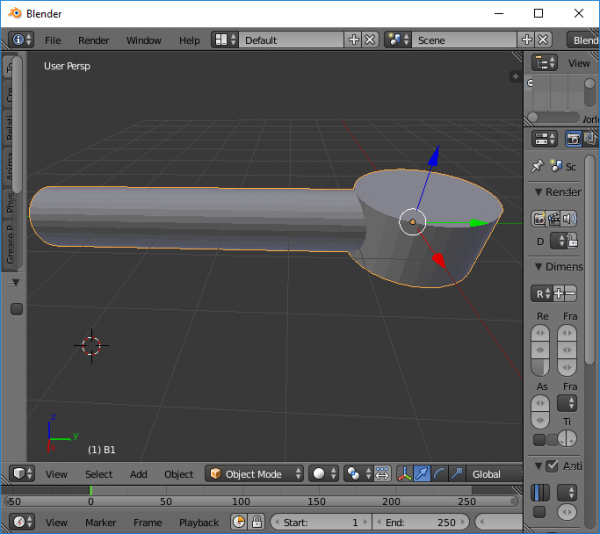
\includegraphics[width=7cm]{11.png}
\caption{Diseño incorrecto de eslabón 1.}
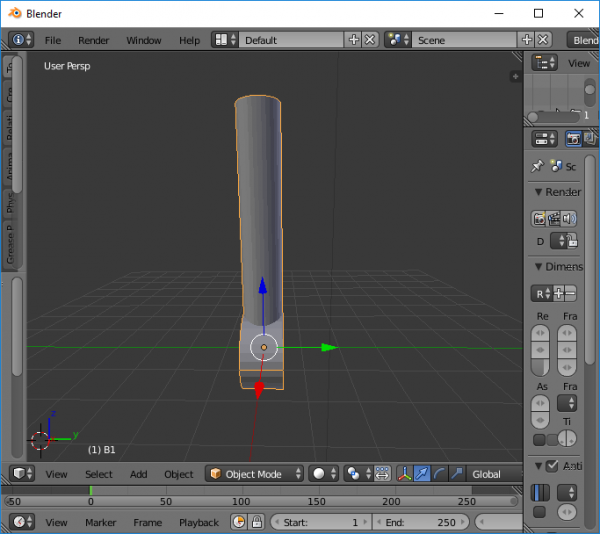
\includegraphics[width=7cm]{12.png}
\caption{Diseño correcto de eslabón 1. El eje z coincide con el eje de la articulación A2 al ensamblar el robot.}
\end{figure}

De esta forma, al esamblar el robot,  el eje z local del eslabón 1 coincide con la dirección el eje de la articulación $A_{2}$ como se ilustra en la f¡gura 6 y el eje x queda como ya se había establecido (figura 8). Continuando este procedimiento para cada eslabon, el sistema de referencia local en cada eslabón debe ser como se muestra en la figura 13.

\begin{figure}[hbtp]
\centering
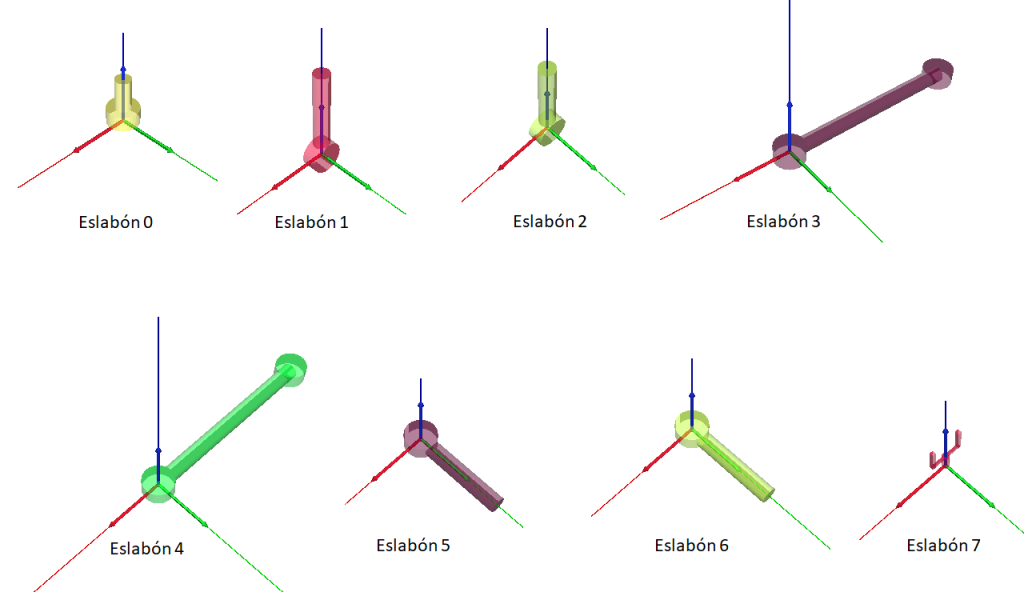
\includegraphics[width=9cm]{13.png}
\caption{Sistema de referecia local apropiado, intente ensamblar el robot cumpliendo con loas pasos anteriores y note que el resultado es como el de la figura 14. No es necesario hacer todo el ensamble mentalmente, hágalo con cada par de eslabones contiguos, recuerde que el eje z de cada eslabón es el eje de rotación alrededor del cual rota el siguiente eslabón.}
\end{figure}
\subsection{Paso 3}
\textbf{Determinar la dirección de los ejes} $y_{i}$.
El eje $y_{i}=z_{i}X x_{i}$.
\begin{figure}[hbtp]
\centering
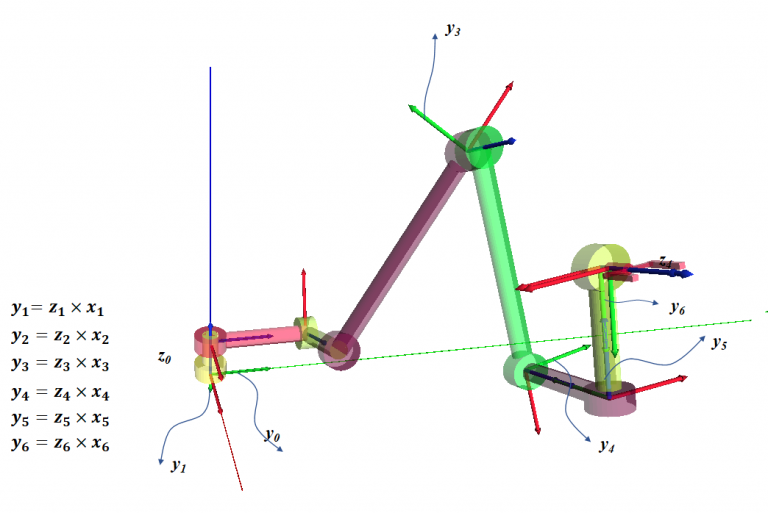
\includegraphics[width=8cm]{14.png}
\caption{Elección de la dirección de los ejes y para formar sistemas que obdezcan a la regla de la mano derecha.}
\end{figure}
\subsubsection{Descripción de las transformaciones}
Es natural que durante el diseño se deseen conocer las dimensiones de cada eslabón, así también la forma deben rotar los sistemas de referencia de cada eslabón para que las orientaciones resultantes  cumplan con la convención DH; esto es precisamente una tarea que debe realizarse antes de realizar la simulación o animación; existen un conjunto de parámetros que caracterizan la configuración DH de un robot y son precisamente los que permiten realizar un ensamble que cumpla con el algoritmo DH, dichos parámetros que conforman un sistema de coordenadas, llamado sistema de coordenadas DH, son los que debemos medir para poder construir la simulación que ejecute una cinemática directa del robot.

Para referencia se ilustran las medidas (sin unidades) de los eslabones.
\begin{figure}[hbtp]
\centering
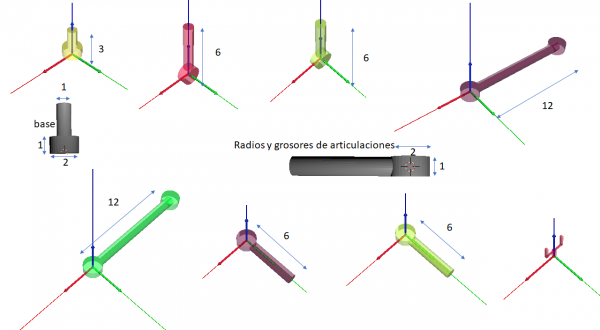
\includegraphics[width=9cm]{15.png}
\caption{Dimensiones de los eslabones}
\end{figure}
Para referencia nos apoyamos  en la figuras   15 y 16.
\begin{figure}[hbtp]
\centering
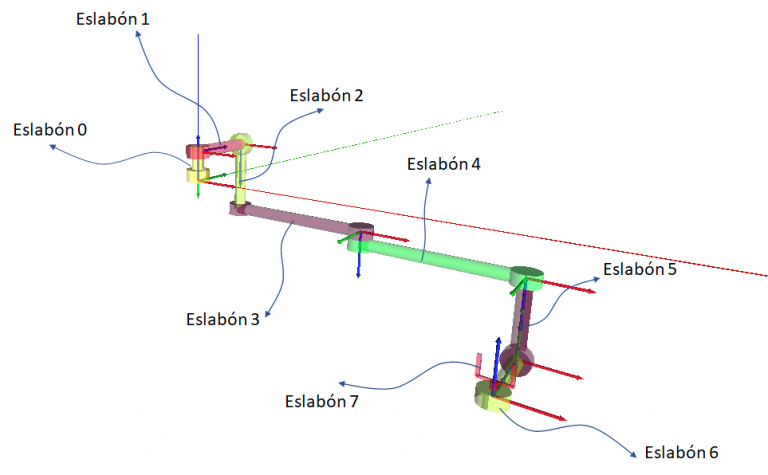
\includegraphics[width=9cm]{16.png}
\caption{Configuración DH}
\end{figure}

Para describir las transformaciones que sufre cada eslabón, nos concetraremos en los  ejes de cada eslabón en forma individual y en el eslabón siguiente que se muestran en la figura 16 (no en figura 14, ya que esa figura representa al robot cuando ya se han realizado rotaciones alrededor de algunos de los ejes z), analizamos los cambios de orientación entre los sistemas de referencia de un eslabón y su sucesor. Lo interesante de la convención DH es que el cambio de orientación de un sistema de referencia está dado por el producto de dos transformaciones homogéneas que tienen la forma simplificada
\begin{figure}[hbtp]
\centering
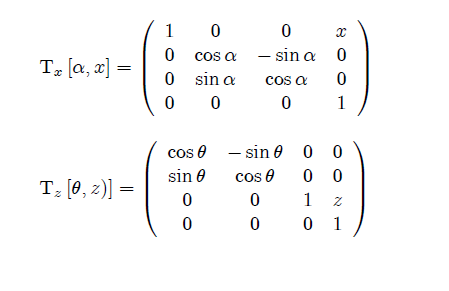
\includegraphics[width=5cm]{17.png}
\caption{Forma de las transformaciones homogéneas que experimenta cada eslabón en una configuración DH}
\end{figure}
y dado que en nuestro caso de estudio hay 8 eslabones la posición(r)respecto del sistema de referencia global de un punto (rp)medido en el sistema de referencia del efector final está dado por.
\begin{center}
$T(r)=T_{0}*T_{1}*T_{2}*T_{3}*T_{4}*T_{5}*T_{6}*T_{7}(rp)$
\end{center}

Donde cada $T_{i}$ con i=1,2,3,4,5,6,7 está dada por el producto de dos transformaciones homogéneas que tienen la forma:
\begin{center}
$T_{i}=T_{zi-1}[\theta_{i},z]*Tx_{xi-1}[\alpha_{1},x]$
\end{center}
En codigo fuente se expresa:

\centering
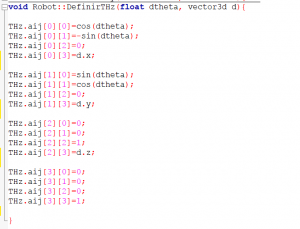
\includegraphics[scale=1]{18.png}
 
 \section{Referencias}
 @article{barrientos2012modelado,
  title={Modelado de Caden as Cinem{\'a}ticas mediante Matrices de Desplazamiento. Una alternativa al m{\'e}todo de Denavit-Hartenberg},
  author={Barrientos, A and {\'A}lvarez, M and Hern{\'a}ndez, JD and Del Cerro, J and Rossi, Claudio},
  journal={Revista Iberoamericana de Autom{\'a}tica e Inform{\'a}tica industrial},
  volume={9},
  number={4},
  pages={371--382},
  year={2012}
\cite{barrientos2012modelado}
\bibliographystyle{apalike} 
\bibliography{biblio}

\end{document}